\documentclass[grad,numbers]{coppe}
\usepackage[utf8]{inputenc}
\usepackage{amsmath,amssymb}
\usepackage{hyperref}

\makelosymbols
\makeloabbreviations



  \RequirePackage[english, brazil]{babel}


\providecommand{\tightlist}{%
  \setlength{\itemsep}{0pt}\setlength{\parskip}{0pt}}
\usepackage{longtable}
\usepackage{booktabs}
\begin{document}
  \title{\emph{Valuation} Intrínseco e Relativo: O estudo de caso da COPEL}
  \foreigntitle{Intrinsic and Relative Valuation: The case study of COPEL}
    \author{Rafael Pinto}{de Freitas}
  
    \advisor{Prof.}{José Roberto}{Ribas}{D.Sc.}
    \advisor{Prof.}{Nome do Segundo Orientador}{Sobrenome}{Ph.D}
  

    \examiner{Prof.}{José Roberto Ribas}{D.Sc.}
    \examiner{Prof.}{Nome Completo do Segundo Examinador}{Ph.D}
    \examiner{Prof.}{Nome Completo do Terceiro Examinador}{Ph.D}
  
  \department{EPR}
  \date{08}{2020}

    \keyword{Valuation}
    \keyword{Análise de investimentos}
  
  \maketitle

  \frontmatter
  \dedication{\begin{quote}
Judge a man by his questions rather than by his answers.

\hfill --- Voltaire
\end{quote}}
    \chapter*{Agradecimentos}
  Agradeço pela oportunidade de cursar um ensino superior de qualidade de forma pública. Mesmo com suas diversas limitações e imperfeições, a República brasileira segue em frente com a mensagem de democratização do conhecimento. É somente por meio desta que podemos nos defender contra a tirania vil da ignorância. Dessa forma, estou em dívida com a sociedade; com todos que permitiram minha entrada e estadia no curso de Engenharia de Produção pela UFRJ. Uma dívida monumental, se pensada pela ótica dos benefícios. Espero retornar o investimento em breve, a começar de forma humilde com este trabalho de conclusão de curso. Boa leitura!
  \begin{abstract}
Sit urna lacus aenean euismod morbi integer mauris ligula euismod. Massa leo nunc rutrum non vulputate viverra erat aliquet torquent. Dictumst inceptos litora diam dui eu non sodales eget metus? Mollis faucibus justo class class nulla vestibulum consequat purus.

Sit est ligula massa massa. Lectus parturient vehicula luctus nisl facilisis iaculis sagittis euismod ornare ut platea! Vestibulum et cras nostra luctus morbi cubilia et ante ornare luctus commodo facilisis nam. Lobortis ligula dictum tortor facilisis ante gravida habitasse cras laoreet. Vehicula pharetra vulputate non magna ut interdum habitant quam et class elementum arcu!

Adipiscing nulla laoreet magna dignissim nostra phasellus lacinia elementum est id! Rutrum arcu aliquet torquent porttitor ligula eget dictumst aenean. Lacus dictumst phasellus sed lobortis leo convallis velit mi imperdiet. Ultricies convallis id vestibulum morbi rutrum tortor diam volutpat euismod montes enim cras eros luctus duis rutrum integer.

Consectetur platea augue vitae vitae integer ad tincidunt torquent ac. Pharetra malesuada odio non lobortis dis aliquet arcu nascetur magna porttitor. Lacinia curabitur primis ligula magna sociosqu hendrerit sociosqu risus cubilia. Arcu potenti mi pellentesque nulla per varius vitae lectus pellentesque! Tempor.
  \end{abstract}
  \begin{foreignabstract}
Sit urna lacus aenean euismod morbi integer mauris ligula euismod. Massa leo nunc rutrum non vulputate viverra erat aliquet torquent. Dictumst inceptos litora diam dui eu non sodales eget metus? Mollis faucibus justo class class nulla vestibulum consequat purus.

Sit est ligula massa massa. Lectus parturient vehicula luctus nisl facilisis iaculis sagittis euismod ornare ut platea! Vestibulum et cras nostra luctus morbi cubilia et ante ornare luctus commodo facilisis nam. Lobortis ligula dictum tortor facilisis ante gravida habitasse cras laoreet. Vehicula pharetra vulputate non magna ut interdum habitant quam et class elementum arcu!

Adipiscing nulla laoreet magna dignissim nostra phasellus lacinia elementum est id! Rutrum arcu aliquet torquent porttitor ligula eget dictumst aenean. Lacus dictumst phasellus sed lobortis leo convallis velit mi imperdiet. Ultricies convallis id vestibulum morbi rutrum tortor diam volutpat euismod montes enim cras eros luctus duis rutrum integer.

Consectetur platea augue vitae vitae integer ad tincidunt torquent ac. Pharetra malesuada odio non lobortis dis aliquet arcu nascetur magna porttitor. Lacinia curabitur primis ligula magna sociosqu hendrerit sociosqu risus cubilia. Arcu potenti mi pellentesque nulla per varius vitae lectus pellentesque! Tempor.
  \end{foreignabstract}
  \tableofcontents

  \listoffigures

  \listoftables

  \printlosymbols
  \printloabbreviations

  \mainmatter

  \hypertarget{introduuxe7uxe3o}{%
  \chapter{Introdução}\label{introduuxe7uxe3o}}
  
  Cabe, antes de começar o desenvolvimento do trabalho propriamente dito, contextualizar e justificar o trabalho, assim como explicitar aos leitores os objetivos, as limitações e a estrutura do mesmo.
  
  \hypertarget{contextualizauxe7uxe3o}{%
  \section{Contextualização}\label{contextualizauxe7uxe3o}}
  
  É necessário definir Bolsas de Valores, assim como retratar uma breve história da brasileira a partir de 1967 -- ano a partir do qual começou a se chamar Bolsa de Valores de São Paulo, a Bovespa. Segundo Assaf Neto (\protect\hyperlink{ref-assafneto2018}{2018}), as Bolsas são entidades, cujo objetivo básico é o de manter um local em condições adequadas para a realização de operações de compra e venda de títulos e valores mobiliários.
  
  Um ano após 1967, foi criado o principal índice de ações brasileiro: o Ibovespa. Resumidamente, este índice é uma média ponderada das ações com maior volume de negociação. Após certo tempo, foi criada a Cetip -- a Central de Custódia e de Liquidação Financeira de Títulos -- em 1984, começando a operar em 1986.
  
  A partir de 2007, as bolsas de valores deixaram de ser entidades sem fins lucrativos e tornaram-se empresas de capital aberto. No ano seguinte, a BM\&F e a Bovespa se uniram, resultando na criação da Bolsa de Valores, Mercadorias e Futuros de São Paulo -- a BM\&F Bovespa. Em 2017, são fundidas a BM\&F Bovespa e Cetip, dando origem à B3 S.A., sob a supervisão da Comissão de Valores Mobiliários -- esta é a bolsa brasileira atualmente.
  
  Em tempos contemporâneos, há um crescimento de CPFs registrados na Bolsa de Valores ano a ano, sendo em 2020 o recorde, um aumento de 47.7\% relativo a maio de 2019\footnote{O último acesso a estes dados foi em 07 jul 2020. Pode-se conferir a evolução dos mesmos baixando a planilha presente neste link: \url{http://www.b3.com.br/pt_br/market-data-e-indices/servicos-de-dados/market-data/consultas/mercado-a-vista/historico-pessoas-fisicas/}}.
  
  Com diversos setores e subsetores de atuação, são diversas as empresas de capital aberto à disposição para escolha do crescente número de investidores brasileiros -- o que não quer dizer que o investidor deve investir em todos. De fato, o investidor precisa minimizar seu risco, preferencialmente investindo em empresas que dentre outras características possuem alto \emph{payout} de dividendos, baixo grau de alavancagem; e menor variabilidade de lucros (BEAVER; KETTLER; SCHOLES, \protect\hyperlink{ref-beaver1970}{1970}).
  
  Empresas do setor de utilidades possuem tais características, em sua maioria; dessa forma, escolheu-se um exemplar do mesmo -- a Companhia Paranaense de Energia, COPEL -- como forma de fazer o valuation da empresa, fazer um breve resumo do setor elétrico e exemplificar o processo ao leitor.
  
  \hypertarget{justificativa}{%
  \section{Justificativa}\label{justificativa}}
  
  Por mais que a caderneta de poupança seja o investimento preferido dos brasileiros, segundo a Associação Brasileira das Entidades dos Mercados Financeiro e de Capitais (\protect\hyperlink{ref-anbima2019}{2019}) -- esta modalidade conta com 88\% da população -- é evidente que o rendimento nominal\footnote{Nominal, pois os retornos reais são contextuais devido ao pagamento de impostos, dividendos; e, a depender do ativo, dos custos do mesmo.} do IBOV é superior no longo prazo. Pelo IPEA, pode-se obter tanto os rendimentos nominais (em \% a.m.) da poupança quanto os retornos do IBOV (também em \% a.m.), ambos em intervalos mensais desde 1990. A partir daí, acumulamos as taxas recursivamente. Definindo \(i\) como a taxa de retorno nominal total, e \(i_t\) como sendo a taxa de retorno nominal no mês \(t\), temos \(i = \prod_{t=1}^n (1+i_t),\) sendo \(n\) o mês que se deseja calcular o retorno nominal total. Exposto isso, foi feito um gráfico dos retornos totais de ambas as modalidades:
  \begin{figure}[H]
  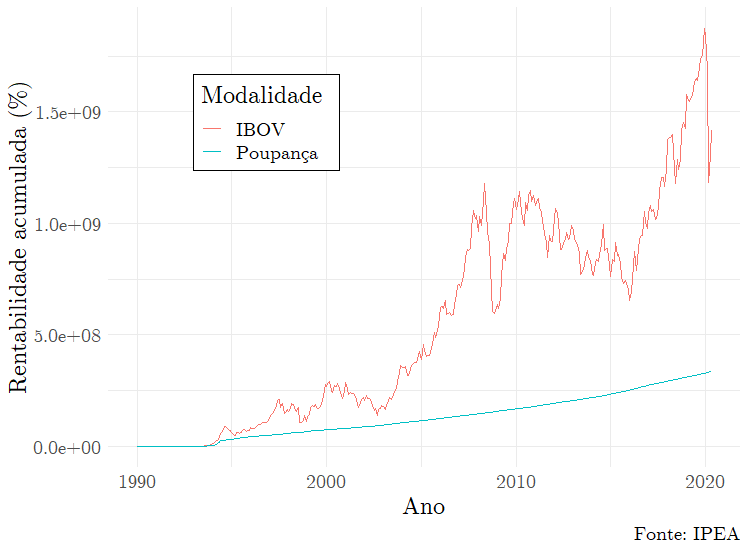
\includegraphics[width=1\linewidth]{img/ibov-poupanca} \caption{Uma comparação entre o IBOV e a poupança.}\label{fig:unnamed-chunk-1}
  \end{figure}
  Com o passar do tempo, entretanto, a maturação no mercado financeiro pode, naturalmente, levar o investidor a se interessar por retornos acima do mercado -- fundos de índice, por definição, impossibilitam o objetivo. Isso leva a uma exploração de diferentes classes de ativos, desde ações ordinárias a fundos de investimento em ações. Um investidor, entretanto, há de ter em mente que raramente fundos de investimento com administração ativa, no longo prazo, superam os retornos dos fundos de índice, em termos reais (BOGLE, \protect\hyperlink{ref-bogle2015}{2015}).
  
  Assim sendo, caso o investidor deseja ter sucesso, é importante que as escolhas de ativos sejam racionais. Ao menos, tão racionais quanto possível forem para humanos. De fato, indivíduos estão sujeitos a uma racionalidade restrita (SIMON, \protect\hyperlink{ref-simon1997}{1997}), o que leva a diversas heurísticas -- inclusive, mas não limitadas a: enfatizar evidências que apoiam visões próprias (KLAYMAN, \protect\hyperlink{ref-klayman1995}{1995}), superestimar probabilidades por maior ``disponibilidade'' em memória (SCHWARZ et al., \protect\hyperlink{ref-schwarz1991}{1991}); e superestimar a própria habilidade, quando se é novato, assim como subestimar, quando se é um \emph{expert} (KRUGER; DUNNING, \protect\hyperlink{ref-kruger1999}{1999}) -- para simplificar o processo de raciocínio e, permitir, assim, que o agente consiga satisfazer as restrições -- tempo, recursos, dentre outros -- para a tomada de decisões.
  
  De fato, a abordagem de realizar tanto o \emph{valuation} intrínseco quanto o relativo de uma empresa é, além de uma interessante comparação entre métodos, uma forma de evitar a ``síndrome do homem com martelo'', popularizado por Munger (\protect\hyperlink{ref-munger2006}{2006}). Este cita um provérbio, que diz: ``Para um homem com um martelo, todo problema se parece com um prego.''
  
  \hypertarget{objetivos}{%
  \section{Objetivos}\label{objetivos}}
  
  São os principais objetivos do trabalho (1) fazer o \emph{valuation} da Companhia Paranaense de Energia através de, no mínimo, dois métodos de valuation, sendo no mínimo um deles intrísenco e no mínimo, um relativo e (2) realizar a comparação entre os resultados dos métodos.
  
  Com o desenvolver do trabalho, poderão ser percebidas outras motivações, entretanto seriam estas consideradas secundárias.
  
  \hypertarget{limitauxe7uxf5es}{%
  \section{Limitações}\label{limitauxe7uxf5es}}
  
  Este trabalho se limita a prover um breve prospecto do cenário energético brasileiro, assim como possíveis desenvolvimentos. Não serão discutidas políticas energéticas e afins. Se limita, também, a tomar como verdadeira a teoria moderna do portfólio como exposta por Markowitz (\protect\hyperlink{ref-markowitz1952}{1952}), para o cálculo do custo de capital. Não será discutido economia comportamental, nem modelos mais sofisticados para tal cálculo.
  
  \hypertarget{estrutura-do-trabalho}{%
  \section{Estrutura do trabalho}\label{estrutura-do-trabalho}}
  
  O trabalho possui, em sua integridade, cinco capítulos.
  
  O primeiro capítulo é uma introdução ao restante do trabalho, e é efetivamente um resumo do que o leitor verá pela frente.
  
  O segundo capítulo é uma examinação do setor energético brasileiro, a ser feito pela leitura e examinação do Plano Decenal de Expansão de Energia (PDE) e o Plano Nacioanl de Energia (PNE), ambos elaborados pela Empresa de Pesquisa Energética (EPE). Através destes, podemos ter uma melhor noção do setor no qual a empresa está inserido, possibilitando um melhor cálculo e previsão dos fluxos de caixa.
  
  O terceiro capítulo é a documentação do referencial teórico utilizado, a ser escrito seguindo uma lógica linear, de forma tal que possa também ser visto como uma metodologia, com exemplos para auxiliar o leitor.
  
  O quarto capítulo é o estudo de caso de fato. Será dada uma contextualização da empresa, assim como a aplicação dos métodos discutidos.
  
  O quinto e último capítulo é a conclusão, em que será feita a exposição dos resultados, assim como a comparação entre os métodos de \emph{valuation} discutidos durante o texto.
  
  \hypertarget{o-mercado-de-energia}{%
  \chapter{O mercado de energia}\label{o-mercado-de-energia}}
  
  É importante, antes de partir para o estudo de caso em questão, estabelecer o contexto do trabalho em questão. De fato, neste capítulo serão tratados os fundamentais do mercado de energia no Brasil, desde os órgãos aos estudos principais do setor.
  
  \hypertarget{uxf3rguxe3os-presentes-no-estudo}{%
  \section{Órgãos presentes no estudo}\label{uxf3rguxe3os-presentes-no-estudo}}
  
  Nesta seção, serão tratados os cinco principais órgãos do setor, sendo eles: (1) o Ministério de Minas e Energia; (2) a Agência Nacional de Energia Elétrica; (3) o Operador Nacional do Sistema Elétrico; (4) a Câmara Comercializadora de Energia Elétrica; e (5) a Empresa de Pesquisa Energética.
  
  \hypertarget{mme}{%
  \subsection{MME}\label{mme}}
  
  O Ministério de Minas e Energia (MME) foi criado em 1960, no governo do presidente Juscelino Kubitschek. Assim seguiu por 30 anos, até ser extinto em 1990 e recriado em 1992.
  
  Em 1997, foi criado o Conselho Nacional de Política Energética (CNPE), vinculado à Presidência da República e presidido pelo ministro de Minas e Energia, com a atribuição de propor ao presidente da República políticas nacionais e medidas para o setor.
  
  Logo em seguida, em 2003, foram definidas as competências do MME como sendo as áreas de (1) geologia, recursos minerais e energéticos; (2) aproveitamento da energia hidráulica; mineração e metalurgia; e (3) petróleo, combustível e energia elétrica.
  
  No ano seguinte foi criado o Comitê de Monitoramento do Setor Elétrico (CMSE), cuja função é acompanhar e avaliar permanentemente a continuidade e a segurança do suprimento eletroenergético em todo o território nacional. No mesmo ano, foi permitida também a criação da Empresa de Pesquisa Energética (EPE), vinculada ao Ministério, que tem por finalidade prestar serviços na área de estudos e pesquisas destinadas a subsidiar o planejamento do setor energético.
  
  O MME tem como empresas vinculadas a Eletrobras e Petrobras. Estão, também, vinculadas algumas autarquias ao Ministério, dentre elas: a Agência Nacional de Energia Elétrica (ANEEL); Agência Nacional do Petróleo, Gás Natural e Biocombustíveis (ANP); e a Agência Nacional de Mineração (ANM).
  
  \hypertarget{aneel}{%
  \subsection{ANEEL}\label{aneel}}
  
  A Agência Nacional de Energia Elétrica (ANEEL) é uma autarquia vinculada ao Ministério de Minas e Energia. Tem como finalidade regular e fiscalizar a produção, transmissão, distribuição e comercialização de energia elétrica, de acordo com a legislação e em conformidade com as diretrizes e as políticas do governo federal.
  
  Cabe à ANEEL, dentre outras competências: (1) implementar as políticas e diretrizes do governo federal para a exploração da energia elétrica e o aproveitamento dos potenciais hidráulicos; (2) estabelecer as tarifas para o suprimento de energia elétrica realizado às concessionárias e permissionárias de distribuição; e (3) fazer a gestão dos contratos de concessão ou de permisão de serviços públicos de energia elétrica e fiscalizar, diretamente ou mediante convênios com órgãos estaduais, as concessões, as permissões e a prestação dos serviços de energia elétrica.
  
  Pode-se conferir a lista completa de atribuições pelo art. 3° da lei n°
  9.427/96.
  
  \hypertarget{ons}{%
  \subsection{ONS}\label{ons}}
  
  \hypertarget{ccee}{%
  \subsection{CCEE}\label{ccee}}
  
  \hypertarget{epe}{%
  \subsection{EPE}\label{epe}}
  
  \hypertarget{o-fluxo-de-energia}{%
  \section{O fluxo de energia}\label{o-fluxo-de-energia}}
  
  \hypertarget{gerauxe7uxe3o}{%
  \subsection{Geração}\label{gerauxe7uxe3o}}
  
  \hypertarget{transmissuxe3o}{%
  \subsection{Transmissão}\label{transmissuxe3o}}
  
  \hypertarget{comercializauxe7uxe3o}{%
  \subsection{Comercialização}\label{comercializauxe7uxe3o}}
  
  \hypertarget{distribuiuxe7uxe3o}{%
  \subsection{Distribuição}\label{distribuiuxe7uxe3o}}
  
  \hypertarget{estudos-e-projeuxe7uxf5es-de-longo-prazo}{%
  \section{Estudos e projeções de longo prazo}\label{estudos-e-projeuxe7uxf5es-de-longo-prazo}}
  
  \hypertarget{plano-decenal-de-expansuxe3o-de-energia-pde}{%
  \subsection{Plano Decenal de Expansão de Energia (PDE)}\label{plano-decenal-de-expansuxe3o-de-energia-pde}}
  
  \hypertarget{plano-nacional-de-energia-pne}{%
  \subsection{Plano Nacional de Energia (PNE)}\label{plano-nacional-de-energia-pne}}
  
  \hypertarget{referencial-teuxf3rico}{%
  \chapter{Referencial teórico}\label{referencial-teuxf3rico}}
  
  \hypertarget{demonstrauxe7uxf5es-financeiras}{%
  \section{Demonstrações financeiras}\label{demonstrauxe7uxf5es-financeiras}}
  
  \hypertarget{demonstrativo-de-resultados-do-exercuxedcio-dre}{%
  \subsection{Demonstrativo de Resultados do Exercício (DRE)}\label{demonstrativo-de-resultados-do-exercuxedcio-dre}}
  
  \hypertarget{balanuxe7o-patrimonial-bp}{%
  \subsection{Balanço Patrimonial (BP)}\label{balanuxe7o-patrimonial-bp}}
  
  \hypertarget{demonstrativo-de-fluxo-de-caixa-dfc}{%
  \subsection{Demonstrativo de Fluxo de Caixa (DFC)}\label{demonstrativo-de-fluxo-de-caixa-dfc}}
  
  \hypertarget{valuation-intruxednseco}{%
  \section{\texorpdfstring{\emph{Valuation} intrínseco}{Valuation intrínseco}}\label{valuation-intruxednseco}}
  
  \hypertarget{muxe9todo-do-fluxo-de-caixa-descontado}{%
  \subsection{Método do Fluxo de Caixa Descontado}\label{muxe9todo-do-fluxo-de-caixa-descontado}}
  
  \hypertarget{valuation-relativo}{%
  \section{\texorpdfstring{\emph{Valuation} relativo}{Valuation relativo}}\label{valuation-relativo}}
  
  \hypertarget{anuxe1lise-por-muxfaltiplos}{%
  \subsection{Análise por múltiplos}\label{anuxe1lise-por-muxfaltiplos}}
  
  \hypertarget{estudo-de-caso}{%
  \chapter{Estudo de caso}\label{estudo-de-caso}}
  
  \hypertarget{contextualizauxe7uxe3o-da-copel}{%
  \section{Contextualização da COPEL}\label{contextualizauxe7uxe3o-da-copel}}
  
  \hypertarget{histuxf3ria}{%
  \subsection{História}\label{histuxf3ria}}
  
  \hypertarget{core-business}{%
  \subsection{\texorpdfstring{\emph{Core business}}{Core business}}\label{core-business}}
  
  \hypertarget{gerauxe7uxe3o-1}{%
  \subsubsection{Geração}\label{gerauxe7uxe3o-1}}
  
  \hypertarget{transmissuxe3o-1}{%
  \subsubsection{Transmissão}\label{transmissuxe3o-1}}
  
  \hypertarget{distribuiuxe7uxe3o-1}{%
  \subsubsection{Distribuição}\label{distribuiuxe7uxe3o-1}}
  
  \hypertarget{outros}{%
  \subsubsection{Outros}\label{outros}}
  
  \hypertarget{cuxe1lculo-do-valuation-intruxednseco}{%
  \section{\texorpdfstring{Cálculo do \emph{valuation} intrínseco}{Cálculo do valuation intrínseco}}\label{cuxe1lculo-do-valuation-intruxednseco}}
  
  \hypertarget{o-custo-de-capital-muxe9dio-ponderado-wacc}{%
  \subsection{O custo de capital médio ponderado (WACC)}\label{o-custo-de-capital-muxe9dio-ponderado-wacc}}
  
  \hypertarget{custo-de-capital-pruxf3prio}{%
  \subsubsection{Custo de capital próprio}\label{custo-de-capital-pruxf3prio}}
  
  \hypertarget{custo-de-capital-de-terceiros}{%
  \subsubsection{Custo de capital de terceiros}\label{custo-de-capital-de-terceiros}}
  
  \hypertarget{fluxo-de-caixa-descontado}{%
  \subsubsection{Fluxo de caixa descontado}\label{fluxo-de-caixa-descontado}}
  
  \hypertarget{cuxe1lculo-do-valuation-relativo}{%
  \section{\texorpdfstring{Cálculo do \emph{valuation} relativo}{Cálculo do valuation relativo}}\label{cuxe1lculo-do-valuation-relativo}}
  
  \hypertarget{margem-bruta}{%
  \subsection{Margem bruta}\label{margem-bruta}}
  
  \hypertarget{lucros-antes-de-juros-e-impostos-ebit}{%
  \subsection{Lucros antes de juros e impostos (EBIT)}\label{lucros-antes-de-juros-e-impostos-ebit}}
  
  \hypertarget{margem-luxedquida}{%
  \subsection{Margem líquida}\label{margem-luxedquida}}
  
  \hypertarget{razuxe3o-preuxe7olucro-pe}{%
  \subsection{Razão preço/lucro (P/E)}\label{razuxe3o-preuxe7olucro-pe}}
  
  \hypertarget{retorno-sobre-patrimuxf4nio-luxedquido-roe}{%
  \subsection{Retorno sobre patrimônio líquido (ROE)}\label{retorno-sobre-patrimuxf4nio-luxedquido-roe}}
  
  \hypertarget{comparauxe7uxe3o-com-empresas-do-setor}{%
  \subsection{Comparação com empresas do setor}\label{comparauxe7uxe3o-com-empresas-do-setor}}
  
  \hypertarget{conclusuxe3o}{%
  \chapter{Conclusão}\label{conclusuxe3o}}
  
  \backmatter
  
  \hypertarget{referuxeancias-bibliogruxe1ficas}{%
  \chapter*{Referências Bibliográficas}\label{referuxeancias-bibliogruxe1ficas}}
  \addcontentsline{toc}{chapter}{Referências Bibliográficas}
  
  \markboth{References}{References}
  
  \label{bib:begin}
  \noindent
  
  \setlength{\parindent}{-0.20in}
  \setlength{\leftskip}{0.20in}
  \setlength{\parskip}{8pt}
  
  \hypertarget{refs}{}
  \leavevmode\hypertarget{ref-anbima2019}{}%
  ANBIMA. \textbf{Raio-X do Investidor Brasileiro}, 2019.
  
  \leavevmode\hypertarget{ref-beaver1970}{}%
  BEAVER, W.; KETTLER, P.; SCHOLES, M. The association between market determined and accounting determined risk measures. \textbf{The Accounting Review}, v. 45, n. 4, p. 654--682, 1970.
  
  \leavevmode\hypertarget{ref-bogle2015}{}%
  BOGLE, J. C. \textbf{Bogle on mutual funds: New perspectives for the intelligent investor}. New Jersey: John Wiley \& Sons, 2015.
  
  \leavevmode\hypertarget{ref-techreport-exampleIn}{}%
  GARRET, D. A. \textbf{The Microscopic Detection of Corrosion in Aluminum Aircraft Structures with Thermal Neutron Beams and Film Imaging Methods}. Washington, D.C.: National Bureau of Standards, 1977.
  
  \leavevmode\hypertarget{ref-article-example}{}%
  IESAN, D. Existence Theorems in the Theory of Mixtures. \textbf{Journal of Elasticity}, v. 42, n. 2, p. 145--163, fev. 1996.
  
  \leavevmode\hypertarget{ref-klayman1995}{}%
  KLAYMAN, J. Varieties of confirmation bias. \textbf{Psychology of learning and motivation}, v. 32, p. 385--418, 1995.
  
  \leavevmode\hypertarget{ref-kruger1999}{}%
  KRUGER, J.; DUNNING, D. Unskilled and unaware of it: how difficulties in recognizing one's own incompetence lead to inflated self-assessments. \textbf{Journal of personality and social psychology}, v. 77, n. 6, p. 1121, 1999.
  
  \leavevmode\hypertarget{ref-markowitz1952}{}%
  MARKOWITZ, H. Portfolio selection. \textbf{The Journal of Finance}, v. 7, n. 1, p. 77--91, 1952.
  
  \leavevmode\hypertarget{ref-munger2006}{}%
  MUNGER, C. T. \textbf{Poor Charlie's Almanack: The Wit and Wisdom of Charles T. Munger}. Virginia Beach: Donning Company, 2006.
  
  \leavevmode\hypertarget{ref-assafneto2018}{}%
  NETO, A. A. \textbf{Mercado financeiro}. 14. ed. São Paulo: Atlas, 2018.
  
  \leavevmode\hypertarget{ref-schwarz1991}{}%
  SCHWARZ, N. et al. Ease of retrieval as information: another look at the availability heuristic. \textbf{Journal of Personality and Social psychology}, v. 61, n. 2, p. 195, 1991.
  
  \leavevmode\hypertarget{ref-simon1997}{}%
  SIMON, H. A. \textbf{Models of bounded rationality: Empirically grounded economic reason}. Massachusetts: MIT press, 1997. v. 3

  \backmatter
  \bibliographystyle{coppe-unsrt}
  \bibliography{thesis}

  %\appendix
  %\include{appenA}
\end{document}
